\documentclass{article}
\usepackage[english]{babel}
\usepackage[utf8]{inputenc}
% Importing Graphics
\usepackage{graphicx}

\usepackage{listings}

% Colors for code
\usepackage{xcolor}
\definecolor{codegreen}{rgb}{0,0.6,0}
\definecolor{codegray}{rgb}{0.5,0.5,0.5}
\definecolor{codepurple}{rgb}{0.58,0,0.82}
\definecolor{backcolour}{rgb}{0.95,0.95,0.92}

\setlength{\paperwidth}{21cm}   % A4
\setlength{\paperheight}{29.7cm}% A4
\setlength\topmargin{-0.5cm}    
\setlength\oddsidemargin{0cm}   
\setlength\textheight{24.7cm} 
\setlength\textwidth{16.0cm}
\setlength\columnsep{0.6cm}  
\newlength\titlebox 
\setlength\titlebox{5cm}
\setlength\headheight{5pt}   
\setlength\headsep{0pt}
\pagestyle{plain}
\usepackage{color}
\usepackage[natbibapa]{apacite}
\usepackage{xurl}
\usepackage[colorlinks,citecolor=blue,urlcolor=blue, linkcolor=blue, bookmarks=false,hypertexnames=true]{hyperref}
\usepackage{url}
\usepackage{float}
\usepackage{graphicx}
%\usepackage{libertine}
\usepackage{doi} % hyperlink URLs
\renewcommand{\doi}{DOI:~}
% Colors for code
\usepackage{xcolor}
\definecolor{codegreen}{rgb}{0,0.6,0}
\definecolor{codegray}{rgb}{0.5,0.5,0.5}
\definecolor{codepurple}{rgb}{0.58,0,0.82}
\definecolor{backcolour}{rgb}{0.95,0.95,0.92}

\lstdefinestyle{mystyle}{
	commentstyle=\color{codegreen},
	keywordstyle=\color{magenta},
	numberstyle=\tiny\color{codegray},
	stringstyle=\color{codepurple},
	basicstyle=\ttfamily\footnotesize,
	breakatwhitespace=false,         
	breaklines=true,                 
	captionpos=b,                    
	keepspaces=true,                 
	numbers=left,                    
	numbersep=5pt,                  
	showspaces=false,                
	showstringspaces=false,
	showtabs=false,                  
	tabsize=2
}

\lstset{style=mystyle}

\lstdefinestyle{mystyle}{
	commentstyle=\color{codegreen},
	keywordstyle=\color{magenta},
	numberstyle=\tiny\color{codegray},
	stringstyle=\color{codepurple},
	basicstyle=\ttfamily\footnotesize,
	breakatwhitespace=false,         
	breaklines=true,                 
	captionpos=b,                    
	keepspaces=true,                 
	numbers=left,                    
	numbersep=5pt,                  
	showspaces=false,                
	showstringspaces=false,
	showtabs=false,                  
	tabsize=2
}

\lstset{style=mystyle}

\title{CSE 4020 Machine Learning \\ Lab Assessment - 1  }
\author{Sujay Kumar M 20BDS0294\\ \small Computer Science Engineering with Specialization with DataScience\\ \tt sujaykumarreddy.m2020@vitstudent.ac.in
	\\ \url{https://github.com/sujaykumarmag/CSE4020}}



\begin{document}
\maketitle
\section{Making a DataSet}
I made a Laptop with prices Dataset with 3 Columns and 60 rows \\\\\\\
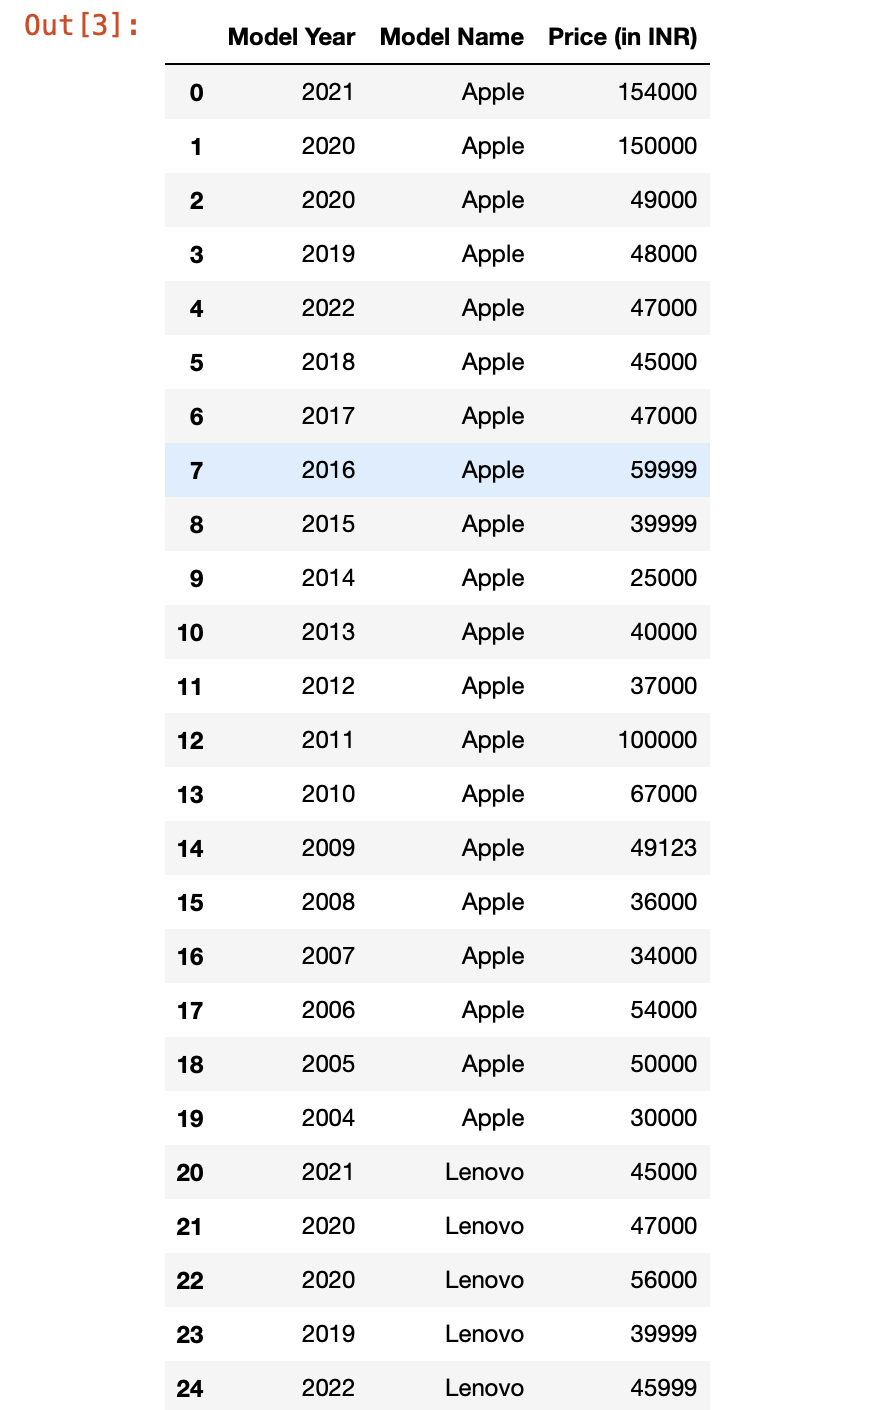
\includegraphics[scale=0.6]{images/1.png}
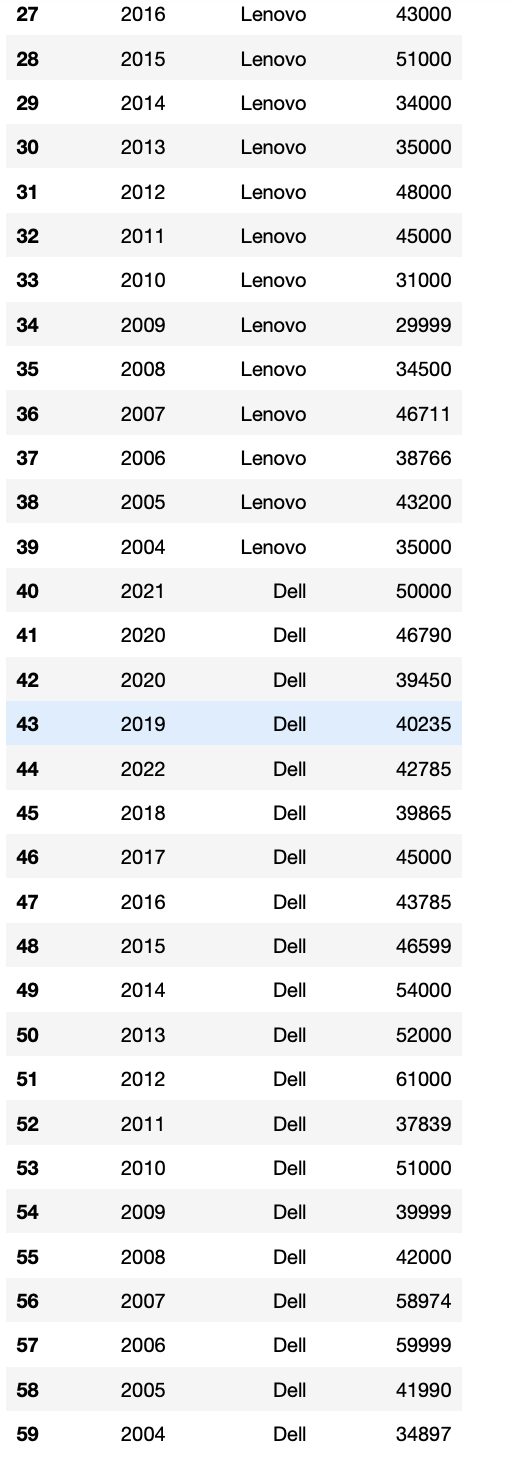
\includegraphics[scale=0.6]{images/2.png}

\section{Data Pre-Processing}
\begin{enumerate}
	\item I used Indexing Order to identify each model name.
	\item For more than 3 attributes its best to use one-hot encoding but multiple regression for different variables is hard to find.
\end{enumerate}

\subsection{Algorithm for Imputing the new column from old column}
\begin{enumerate}
	\item Create an array and append the values according to each row.
	\item Create a new Column and insert it as a dataframe.
	\item Drop the Old Column
\end{enumerate}

\begin{lstlisting}[language=Java]
	
	y = []
	for i in range(len(data)):
		if(data["Model Name"][i]=="Apple"):
			y.append(1)
		elif (data["Model Name"][i] == "Lenovo"):
			y.append(2)
		else:
			y.append(3)
	
	datax = pd.DataFrame(y, columns =['Model Name'])
	x = datax.size
	c = 0
	data["Model Name_opt"] = datax
	while(c<x):
		data["Model Name_opt"].iloc[c]=datax["Model Name"].iloc[c]
		c=c+1
	
	data = data.drop(["Model Name"],axis=1)
	
	
\end{lstlisting}
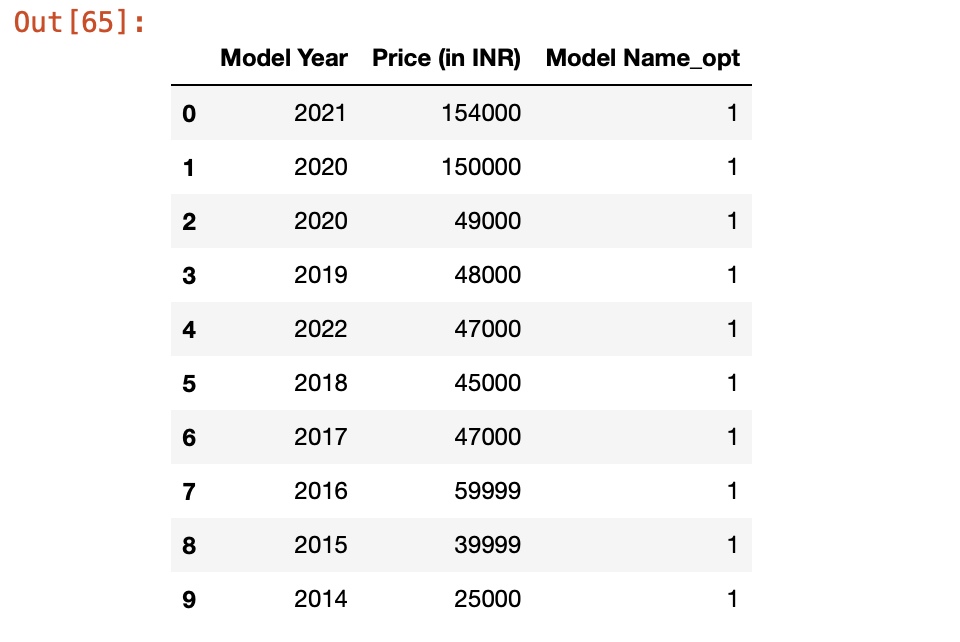
\includegraphics[scale=0.85]{images/3.png}\\\\\\


\section{Multi-Linear Regression (Hot Code)}
\begin{lstlisting}[language=Python]

class Regression:
	# To store the No of dependent variables 
	def __init__(self,no_of_vars):
		self.size = no_of_vars
	
	# Assumption : Only the dependent and target variables are passed separately
	def fit(self,x1,x2,y):
		a = self.double_summation(x2,x2)
		b = self.double_summation(x1,y)
		c = self.double_summation(x1,x2)
		d = self.double_summation(x2,y)
		e = self.double_summation(x1,x1)
		f = c*c
		b1 = ((a*b)-(c*d))/((a*c)-(f))
		b2 = ((e*d)-(c*b))/((a*c)-(f))
		b0 = (y.sum()/self.size)-(b1*(x1.sum()/self.size))-(b2*(x2.sum()/self.size))
		arr = np.array([b0,b1,b2]);
		self.eq = arr
		return arr
	
	# For Printing the Equation
	def __str__(self):
		x = str(self.eq[0][0]) +" + "+str(self.eq[1][0])+"(x1)"+" + "+str(self.eq[2][0])+"(x2)"  
		return x
	
	# This is an Helper Method 
	def double_summation(self,x1,x2):
		sumz = 0
		for i in range(self.size):
			sumz = sumz + (x1[i]*x2[i])
		return sumz
	
	# Assumption : Give me as Numbers not as a np-array
	def predict(self,x1,x2):
		return (self.eq[0]) + ((self.eq[1])*x1) + ((self.eq[2])*x2)    
\end{lstlisting}

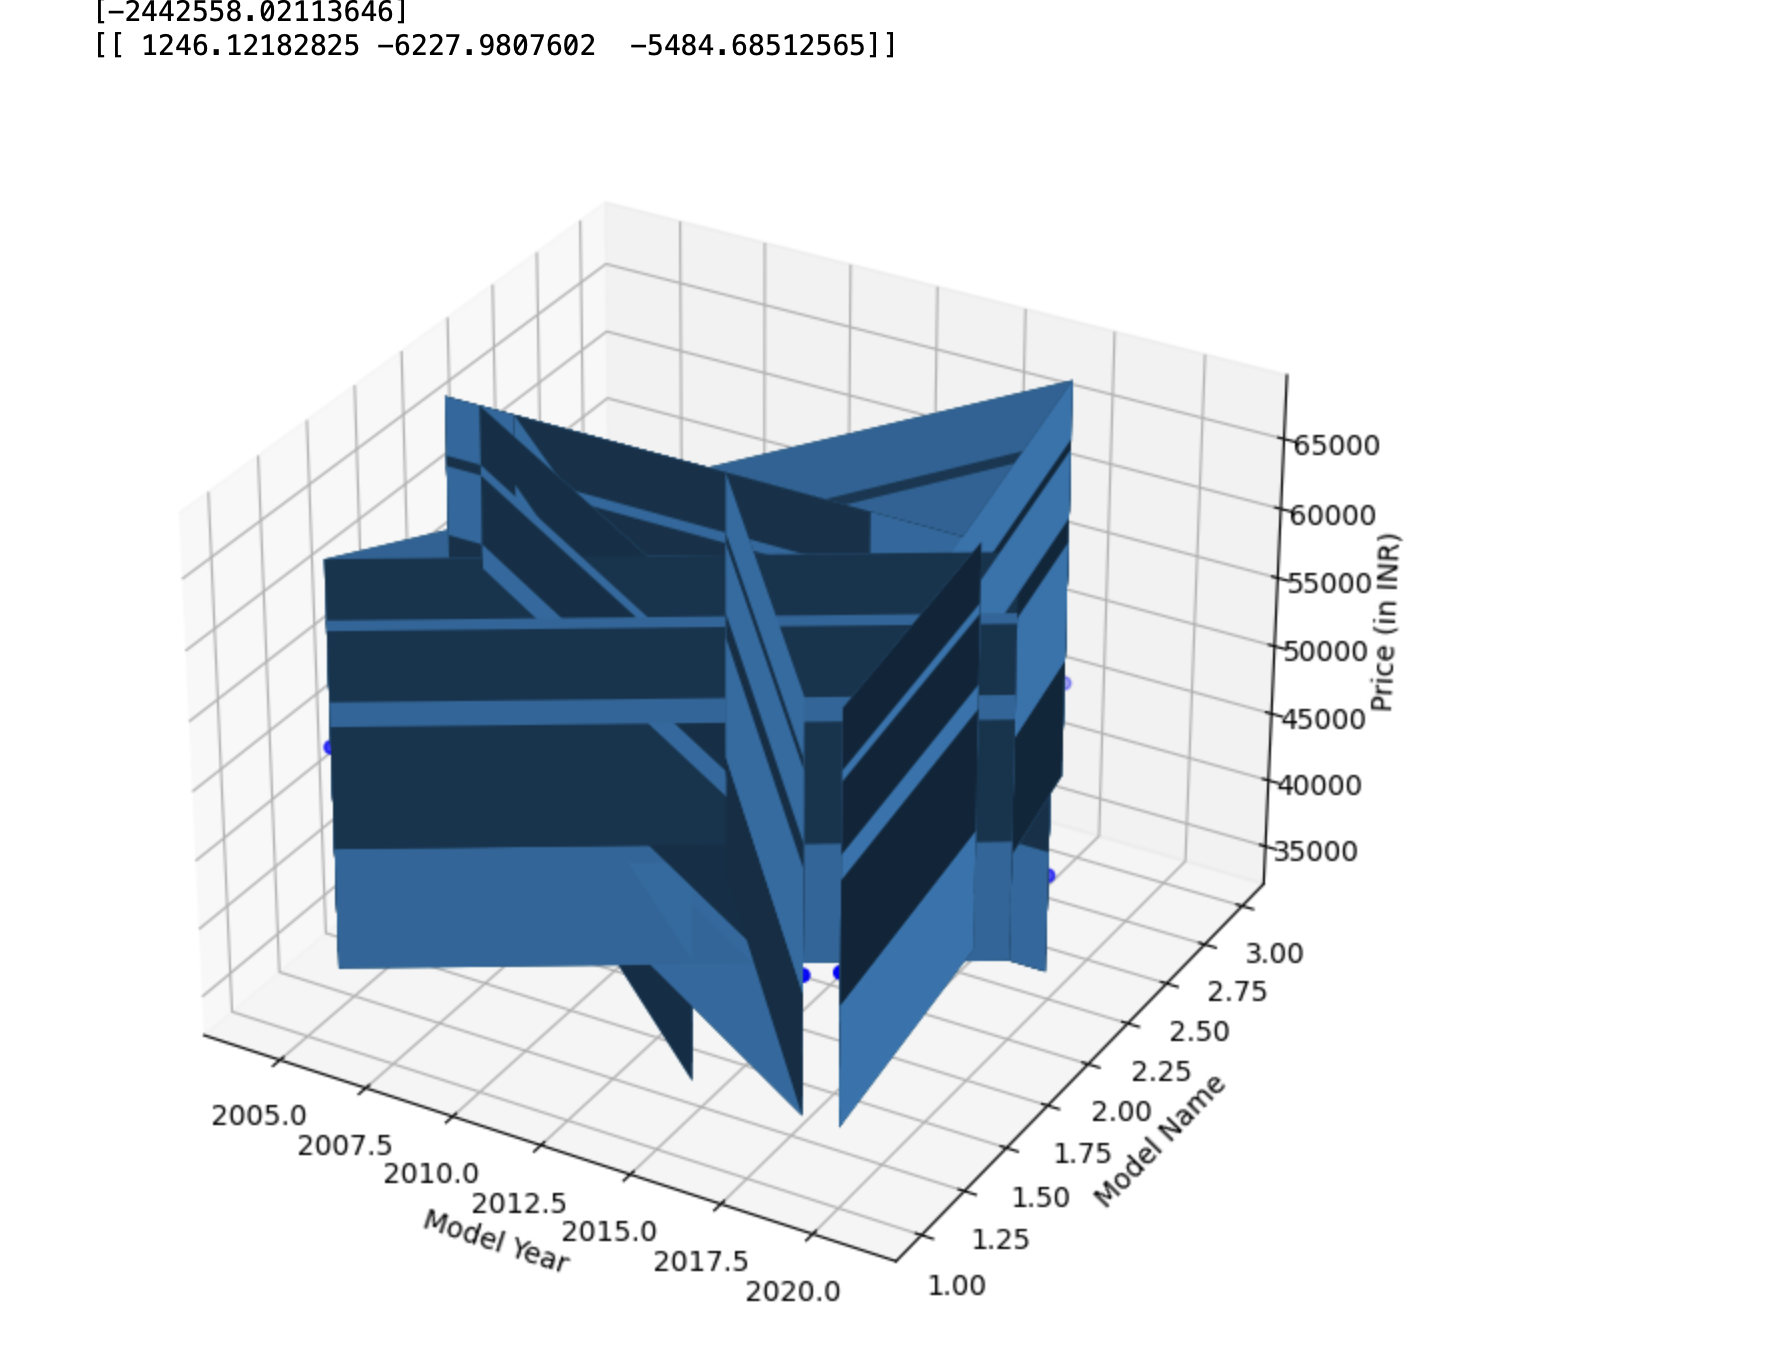
\includegraphics[scale=0.4]{images/4.png}\\\\
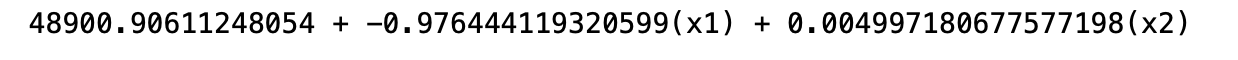
\includegraphics[scale=0.4]{images/5.png}
\\\\

Results Interferred :
\begin{enumerate}
	\item As all the datapoints are covered its known as "Overfitting"
	\item Conclusion : Not a good Algorithm for this Dataset.
\end{enumerate}

\section{Polynomial Regression}
\begin{lstlisting}[language= Python]
	polynomial_features1 = PolynomialFeatures(degree=8)
	x_poly1 = polynomial_features1.fit_transform(X_train)
	model1 = LinearRegression()
	model1.fit(x_poly1, y_train)
	y_poly_pred1 = model1.predict(x_poly1)
	rmse1 = np.sqrt(mean_squared_error(y_train,y_poly_pred1))
	r21 = r2_score(y_train,y_poly_pred1)
	print(rmse1)
	print(r21)
	plt.scatter(X_test.iloc[:,1], y_test, color ='b')
	plt.plot(X_train.iloc[:,1], y_poly_pred1, color ='k')
\end{lstlisting}

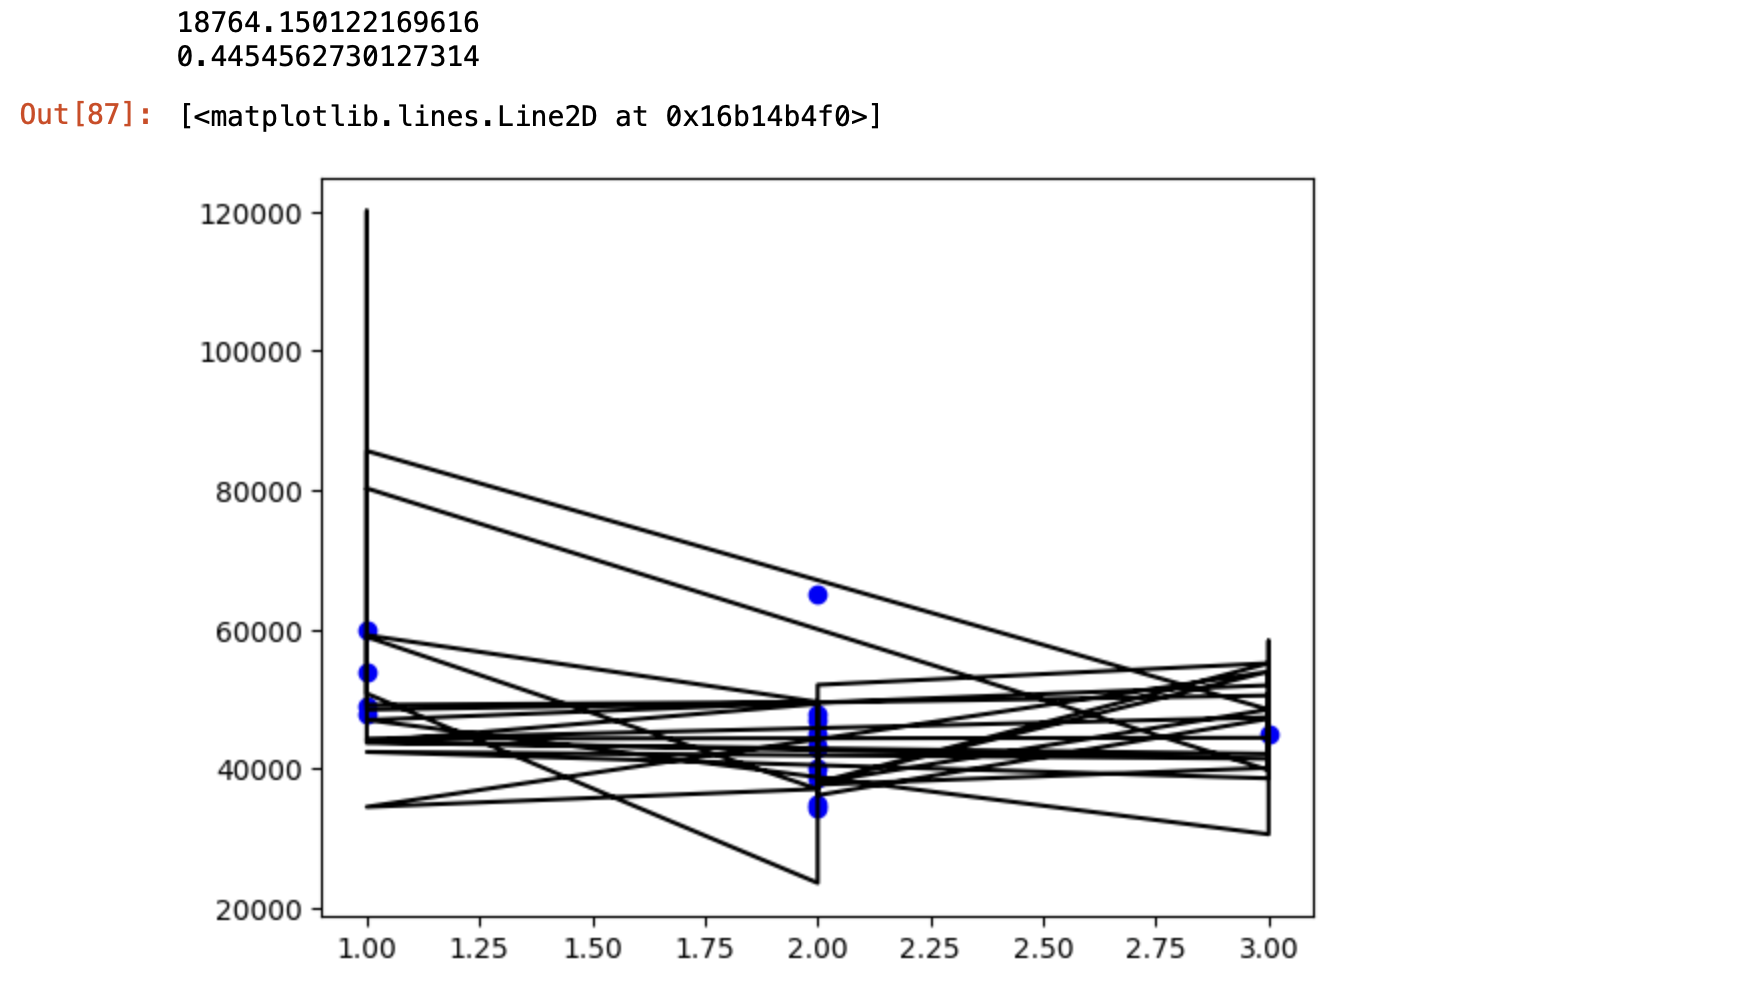
\includegraphics[scale=0.5]{images/6.png}\\\\
Results Interferred :
\begin{enumerate}
	\item As all the datapoints are covered its known as "Overfitting"
	\item The Optimized Degree is 8, after 8 the R\^2 value becomes almost same.
	\item Conclusion : Not a good Algorithm for this Dataset.

\end{enumerate}
	

\section{Logistic Regression}
\subsection{Applying the Class Label}
\begin{enumerate}
	\item Create a new array
	\item Create a new Column in the dataset and insert the column
\end{enumerate}

\begin{lstlisting}[language=Python]
	arr = ["Yes","No","Yes","No","Yes","Yes","No","Yes","Yes","No","Yes","Yes","No","Yes","Yes","No","Yes","Yes","No","Yes","Yes","No","Yes","Yes","No","Yes","Yes","No","Yes","Yes","No","Yes","Yes","No","Yes","Yes","No","Yes","Yes","No","Yes","Yes","No","Yes","Yes","No","Yes","Yes","No","Yes","Yes","No","Yes","Yes","No","Yes","Yes","No","Yes","Yes"]
	
	datax1 = pd.DataFrame(arr, columns =["Buying_Option"])
	x=datax1.size
	c=0
	data["Buy_Option"]=datax1
	while(c<x):
	data["Buy_Option"].iloc[c]=datax1["Buying_Option"].iloc[c]
	c=c+1
	
\end{lstlisting}

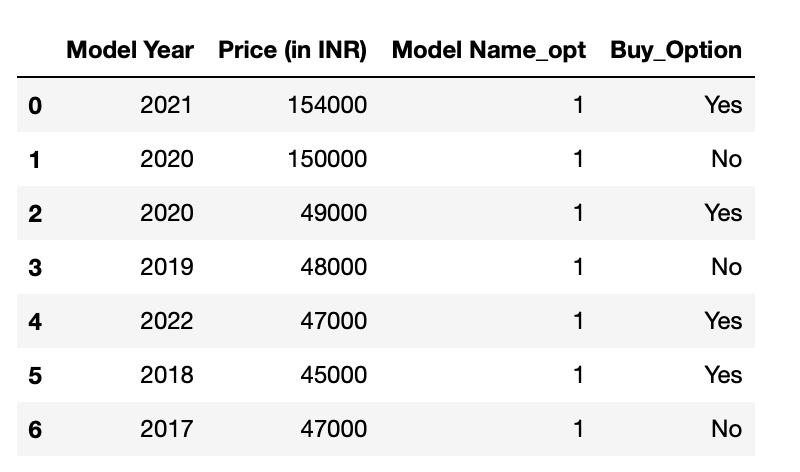
\includegraphics[scale=0.8]{images/7.png}
\subsection{Fitting the Model}
\begin{lstlisting}[language=Python]
	X_train, X_test, y_train, y_test = train_test_split(X, y, test_size = 0.25, random_state = 0)
	
	sc_x = StandardScaler()
	xtrain = sc_x.fit_transform(X_train)
	xtest = sc_x.transform(X_test)
	
	classifier = LogisticRegression(random_state = 0)
	classifier.fit(xtrain, y_train)
	
	y_pred = classifier.predict(xtest)
	
	cm = confusion_matrix(y_test, y_pred)
	
	print ("Confusion Matrix : \n", cm)
	print ("Accuracy : ", accuracy_score(y_test, y_pred))
\end{lstlisting}
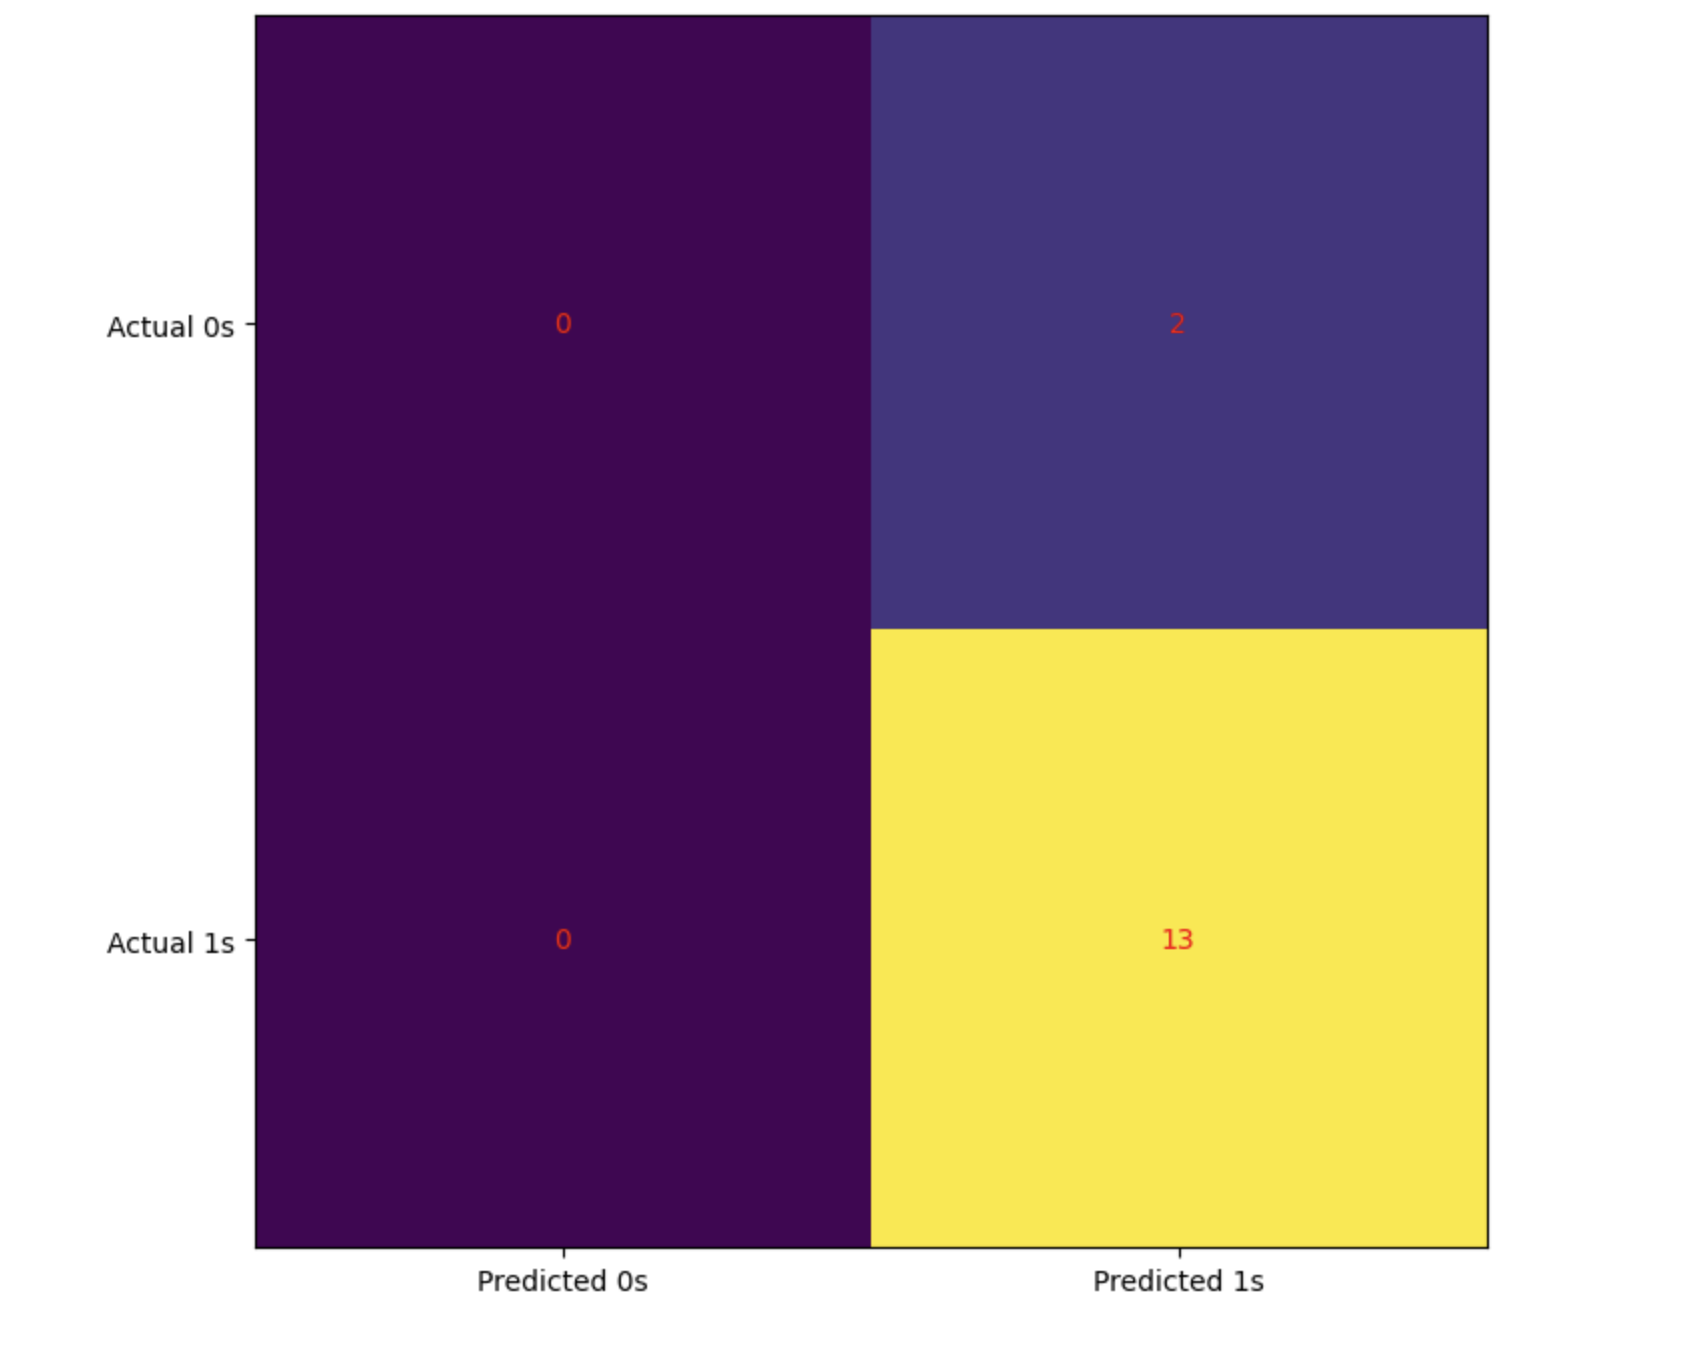
\includegraphics[scale=0.32]{images/8.png}
\end{document}